%%% Local Variables:
%%% mode: latex
%%% TeX-master: t
%%% End:
\documentclass{article}

\usepackage{minted}
\usepackage{graphicx}
\usepackage{appendix}
\usepackage{amsmath}
\usepackage{booktabs}

\graphicspath{ {images/} }

\title{Stochastic Models and Forecasting: Assignment 2}
\author{James Aley}
\date{April 2016}

\begin{document}

\maketitle

\section*{Question 1}

\subsection*{(i)}

The overall mean proportion of days with rainfall is 0.392334. The
R code in Appendix~\ref{apdx:rainfall_preliminary} provides this, plus
proportion of days with rainfall by month over the whole period. It
also creates the plot in Figure~\ref{fig:rainfall_10years} where we've
zoomed in on the most recent 10 year period to make the seasonality
pattern clearer. We can see that the rainfall data have very clear
annual (12 month) seasonality. Higher rainfall can be seen in the
winter months (for the southern hemisphere), and lower values in the
summer each year.

\begin{figure}
  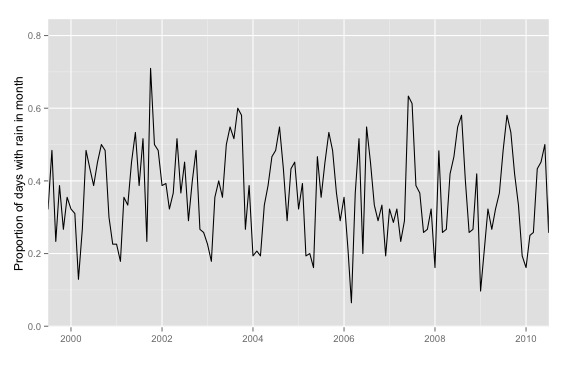
\includegraphics[width=\textwidth]{rainfall_10years}
  \caption{Rainfall proportion by month from January 2000 onward.}\label{fig:rainfall_10years}
  \centering
\end{figure}

\subsection*{(ii)}

The R code in Appendix~\ref{apdx:hmm_fitting} was used to fit models
for \(m = 1, 2, 3\). Note that only the code with the chosen starting
values are shown there for brevity, though many had to be tested in
practice. The estimated parameters for these models are given below.

For \(m = 1 \):

\begin{align*}
  \pi    &= 0.392 \\
  \gamma &= 1 \\
  \delta &= 1 \\
\end{align*}

For \(m = 2\):

\begin{align*}
  \pmb{\pi}    &= \begin{pmatrix} 0.848 \\ 0.000 \end{pmatrix} \\
  \pmb{\Gamma} &= \begin{pmatrix} 0.654 & 0.346 \\
                            0.298 & 0.702 \end{pmatrix} \\
  \pmb{\delta} &= \begin{pmatrix} 0.463 \\ 0.537 \end{pmatrix}
\end{align*}

For \(m = 3\)

\begin{align*}
  \pmb{\pi}    &= \begin{pmatrix} 1.000 \\ 0.000 \\ 0.000 \end{pmatrix} \\
  \pmb{\Gamma} &= \begin{pmatrix} 0.555 & 0.243 & 0.203 \\
                            0.392 & 0.608 & 0.001 \\
                            0.218 & 0.000 & 0.782  \end{pmatrix} \\
  \pmb{\delta} &= \begin{pmatrix} 0.392 \\0.243 \\ 0.365 \end{pmatrix}
\end{align*}

\subsection*{(iii)}


The model with $m = 2$ gives the best fit, as this gives the best score by
BIC and almost the same score as m=3 for AIC.  This can be seen in
Table~\ref{tbl:model_comparison}.

The additional third state in $m=3$ seems to only give a small
improvement in terms of likelihood, but as the growth in parameters is
quadratic in $m$, we see the penalties in AIC and more so in BIC for
adding extra parameters lead us to pick the more parsimonious model.

We can see that we have some natural parameter values in $m = 3$ for
both $\pmb{\Gamma}$ and $\pmb{\pi}$ that are very close to zero and
one. This can cause problems with convergence, and if we truly believe
that a good model for this data should have a third state, we would
probably do better by constraining these parameters to zero or one
respectively, then just estimating the remaining parameters. With no
intuitive basis for this, however, it doesn't seem like a good
approach so we'd probably be better off working with the two-state model.


\begin{table}[]
  \centering
  \begin{tabular}{l l l l}
    \toprule
    $m$ & Negative Log-Likelihood & AIC       & BIC      \\
    \midrule
    1   & 9785.496                & 19572.99  & 19580.58 \\
    2   & 9254.946                & 18517.89  & 18548.25 \\
    3   & 9249.611                & 18517.22  & 18585.53 \\
    \bottomrule
  \end{tabular}
  \caption{HMM Model Comparisons}\label{tbl:model_comparison}
\end{table}

\subsection*{(iv)}

Table~\ref{tbl:hmm_decoding} provides a summary of the first few lines
of output with local and global decoding added as columns to the data
frame. The R code can be found in Appendix~\ref{apdx:hmm_decoding}.

\begin{table}[]
  \centering
  \begin{tabular}{llllll}
    \toprule
    Year & Month & Day & Rain & Local Decoding & Global Decoding \\
    \midrule
    1971 & 1     & 1   & 1    & 1              & 1       \\
    1971 & 1     & 2   & 1    & 1              & 1       \\
    1971 & 1     & 3   & 1    & 1              & 1       \\
    1971 & 1     & 4   & 1    & 1              & 1       \\
    1971 & 1     & 5   & 1    & 1              & 1       \\
    1971 & 1     & 6   & 0    & 3              & 3       \\
    1971 & 1     & 7   & 0    & 3              & 3       \\
    1971 & 1     & 8   & 0    & 3              & 3       \\
    1971 & 1     & 9   & 0    & 3              & 3       \\
    1971 & 1     & 10  & 0    & 3              & 3       \\
  \bottomrule
  \end{tabular}
  \caption{Output summary for local and global decoding}\label{tbl:hmm_decoding}
\end{table}

\subsection*{(v)}

The last few lines of Appendix~\ref{apdx:hmm_decoding} compares the
values of local and global decoding computationally to confirm that
their output is in fact the same. Table~\ref{tbl:hmm_decoding} is
consistent with this.

State 2 is emitted for 3916 of the 14610 data points. Again, the R
code to find these states and create the required data frame can be
seen in Appendix~\ref{apdx:hmm_decoding}. Table~\ref{tbl:hmm_state_2}
shows the first 20 instances of this.

\begin{table}[]
  \centering
  \begin{tabular}{lllllll}
    \toprule
    Observation & Year & Month & Day & Rain & Local Decoding & Global Decoding \\
    \midrule
    26          & 1971 & 1     & 26  & 0    & 2              & 2               \\
    28          & 1971 & 1     & 28  & 0    & 2              & 2               \\
    33          & 1971 & 2     & 2   & 0    & 2              & 2               \\
    36          & 1971 & 2     & 5   & 0    & 2              & 2               \\
    37          & 1971 & 2     & 6   & 0    & 2              & 2               \\
    38          & 1971 & 2     & 7   & 0    & 2              & 2               \\
    39          & 1971 & 2     & 8   & 0    & 2              & 2               \\
    53          & 1971 & 2     & 22  & 0    & 2              & 2               \\
    72          & 1971 & 3     & 13  & 0    & 2              & 2               \\
    73          & 1971 & 3     & 14  & 0    & 2              & 2               \\
    83          & 1971 & 3     & 24  & 0    & 2              & 2               \\
    84          & 1971 & 3     & 25  & 0    & 2              & 2               \\
    87          & 1971 & 3     & 28  & 0    & 2              & 2               \\
    88          & 1971 & 3     & 29  & 0    & 2              & 2               \\
    89          & 1971 & 3     & 30  & 0    & 2              & 2               \\
    111         & 1971 & 4     & 21  & 0    & 2              & 2               \\
    113         & 1971 & 4     & 23  & 0    & 2              & 2               \\
    114         & 1971 & 4     & 24  & 0    & 2              & 2               \\
    115         & 1971 & 4     & 25  & 0    & 2              & 2               \\
    117         & 1971 & 4     & 27  & 0    & 2              & 2 \\
    \bottomrule
  \end{tabular}
  \caption{Rows where Global Decoding is in State 2}\label{tbl:hmm_state_2}
\end{table}

\section*{Question 2}

\subsection*{(i)}

The SAS code provided in Appendix~\ref{apdx:lat_arima} fits simple
ARIMA models to each of the \texttt{avg} and \texttt{end}
variables. For both variables sets, it is easy to say that the data
are not stationary, as we have a clear trend. Differencing the data
once in both case seems to gives us something resembling stationarity
in both cases, with zero means.

For the \texttt{avg} variable, the ARIMA(1, 1, 0) has been chosen. The
sharp cut-off in the PACF at the first lag and significant correlation
at lag one in the ACF give us the ``AR(1) suggesting'' the model will
fit well. After fitting, the portmanteau statistics give us no
significant values and we have no correlation in residuals. All
normality tests for residuals also appear adequate. The fitted model
equation is as follows:

\[
  (1 - 0.29972L) (1 - L) \Delta Y_t = \epsilon_t
\]

For \texttt{end}, the ARIMA(0, 1, 0) has been chosen. After
differencing once we see no significant autocorrelations beyond lag
zero, suggesting that the process is already white noise without any
AR or MA terms to correct it. Further the intercept is fitted to be
very close to zero, so asking SAS not to include an intercept term
slightly further improves the model. Again, we see no significant
residual autocorrelations and the portmanteau statistics have no
significant values. The fitted model equation is given by:

\[
  (1 - L) \Delta Y_t = \epsilon_t
\]

\subsection*{(ii)}

The R code in Appendix~\ref{apdx:lat_var} has been used to fit a
VAR(5) model to the (differenced) data. Fitted model parameters are
given as follows:

\begin{align*}
  \Delta y_t &= \begin{pmatrix} 0.059 & 0.088 \\
                                0.912 & -0.561 \end{pmatrix}
                \begin{pmatrix} \Delta x_{t-1} \\
                                \Delta y_{t-1} \end{pmatrix} \\
             &+ \begin{pmatrix} 0.163 & -0.344 \\
                                0.596 & -0.746  \end{pmatrix}
                \begin{pmatrix} \Delta x_{t-2} \\
                                \Delta y_{t-2} \end{pmatrix} \\
             &+ \begin{pmatrix} 0.292 & -0.178 \\
                                0.605 & -0.445 \end{pmatrix}
                \begin{pmatrix} \Delta x_{t-3} \\
                                \Delta y_{t-3} \end{pmatrix} \\
             &+ \begin{pmatrix} 0.0791 & -0.176 \\
                                0.280 & -0.268  \end{pmatrix}
                \begin{pmatrix} \Delta x_{t-4} \\
                                \Delta y_{t-4} \end{pmatrix} \\
             &+ \begin{pmatrix} 0.139 & -0.030 \\
                                0.242 & -0.046  \end{pmatrix}
                \begin{pmatrix} \Delta x_{t-5} \\
                                \Delta y_{t-5} \end{pmatrix} \\
             &+ \epsilon_t \\
\end{align*}

Table~\ref{tbl:var_portmanteau} summarizes the Portmanteau Statistics
for this model. As we can see, all values but for the highest lags are
significant at the 5\% level, so we conclude that this model does not
fit the data especially well.

Forecasts for the next three months require making use of the
\texttt{predict} function, as shown in the latter part of the code
listing in Appendix~\ref{apdx:lat_var}, then integrating from the
initial starting value, as our model is of differences. The forecasts
for the first three months of 2006 given by this model are 0.587,
0.589 and 0.590.


\begin{table}[]
  \centering
  \begin{tabular}{llll}
    \toprule
    Lags & Statistic & df       & p-value     \\
    \midrule
    5    & 8.946211  & 0.00000  & 0.000999001 \\
    10   & 24.448968 & 11.42857 & 0.000999001 \\
    15   & 41.469536 & 26.45161 & 0.010989011 \\
    20   & 57.767384 & 41.46341 & 0.018981019 \\
    25   & 72.615234 & 56.47059 & 0.037962038 \\
    30   & 88.362401 & 71.47541 & 0.057942058 \\
    \bottomrule
  \end{tabular}
  \caption{Portmanteau Statistics for VAR(5) Lat/Dollar Model}\label{tbl:var_portmanteau}
\end{table}


\begin{appendices}

\subsection*{(iii)}

The SAS code listing in Appendix~\ref{apdx:lat_tfm} fits a transfer
function model to the data. The chosen model has the equation:

\[
  \Delta Y_t = \frac{0.586L}{1 + 0.224L} \Delta X_t + \epsilon_t
\]

We saw earlier that after differencing, the \texttt{end} variable
already exhibits stationarity with no further correction. It was
therefore not necessary to perform any pre-whitening steps. The
cross-correlation function shows high values at lags zero and one,
where we see a sharp cut-off, suggesting the time delay of one lag
required is appropriate.

The portmanteau statistics give us no values close to being
significant, and actually our transfer function model gives us better
AIC and SBC values than any of the previously fitted models.

Forecasts for the first three months of 2006 using this model are
0.5903, 0.5909 and 0.5907.

\section{R Code Listings}

\subsection{Rainfall Data Preliminaries}\label{apdx:rainfall_preliminary}

\begin{minted}{R}
# Install ggplot if it's not already available
install.packages('ggplot2')
require(ggplot2)
library(scales)

## Load data from text file
rainfall <- read.table("data/MelbourneAirport.txt", header=T)
rainfall$date <- as.Date(ISOdate(rainfall$Year, rainfall$Month, rainfall$Day))

## Average rainfall by month:
monthly.rainfall <- aggregate(Rain ~ Year + Month, data=rainfall, FUN=mean)
monthly.rainfall$date <- as.Date(ISOdate(monthly.rainfall$Year,
                                         monthly.rainfall$Month, 1))

# plot to check for seasonality
rainfall.plot <- ggplot(monthly.rainfall, aes(x=date, y=Rain)) +
  geom_line() +
  scale_x_date(labels = date_format("%b %Y")) +
  xlab("") +
  ylab("Proportion of days with rain in month")

rainfall.plot

# Zoom in on recent years to make seasonal pattern more clear
rainfall.plot + xlim(c(as.Date(ISOdate(2000, 1, 1)),
                       as.Date(ISOdate(2010, 1, 1))))
\end{minted}

\subsection{HMM Fitting}\label{apdx:hmm_fitting}

\begin{minted}{R}
# Load the fitting code from lectures
source('hmm_fitting.R')

# Fit models
rainfall.mle1 <- binary.HMM.mle(rainfall$Rain, 1, 0.99, 0.99)
rainfall.mle2 <- binary.HMM.mle(rainfall$Rain, 2,
                                c(0.9, 0.1),
                                matrix(c(0.9, 0.1,
                                         0.1, 0.9),
                                       nrow = 2))
rainfall.mle3 <- binary.HMM.mle(rainfall$Rain, 3,
                                c(0.7, 0.2, 0.1),
                                matrix(c(0.7, 0.2,  0.1,
                                         0.2, 0.7, 0.1,
                                         0.1,  0.2, 0.7),
                                       nrow = 3))
\end{minted}

\subsection{HMM Decoding}\label{apdx:hmm_decoding}

\begin{minted}{R}
# Perform local decoding for 3-state model
local.decoding.3 <- binary.HMM.local_decoding(rainfall$Rain,
                                              3,
                                              rainfall.mle3$pi,
                                              rainfall.mle3$gamma)

# Perform global decoding for 3-state model
global.decoding.3 <- binary.HMM.viterbi(rainfall$Rain,
                                        3,
                                        rainfall.mle3$pi,
                                        rainfall.mle3$gamma)

# Add to data frame
rainfall$local3 <- local.decoding.3
rainfall$global3 <- global.decoding.3

head(rainfall, n = 20)

mean(rainfall$local3 == rainfall$global3)
# == 1, therefore the local and global decodings are the same

# median value for pi is pi2, therefore table for global decoded state = 2:
state.2 <- rainfall[rainfall$global3 == 2, ]
head(state.2, n = 20)
\end{minted}

\subsection{VAR(p) Fitting for Lat/Dollar Data}\label{apdx:lat_var}

\begin{minted}{R}
# Load data
latdol.df <- read.table("~/Downloads/LatDol2.dat",
                        header=F,
                        col.names = c("year", "month", "avg", "end"))

# Create the time series object
end.avg <- data.frame(dend=diff(latdol.df$end),
                      davg=diff(latdol.df$avg))
end.avg.ts <- ts(end.avg)

# Visualise first order differences
plot(end.avg.ts)

# Fit model
ae.ar <- ar(end.avg.ts, order.max = 10)

# Pull in portes package to perform Portmanteau tests
require(portes)
portest(ae.ar)

# Produce forecasts 3 months ahead
p <- predict(ae.ar, n.ahead=3)

p.davg <- c(end.avg.ts[,2], p$pred[,2])
p.avg <- diffinv(p.davg, xi=latdol.df$avg[1])
\end{minted}

\section{SAS Code Listings}

\subsection{Simple ARIMA Models}\label{apdx:lat_arima}

\begin{minted}{text}
/* configure date format */
date = mdy(month, 1, year);
format date MMYYS.;

/* time series visualisations for raw data, unmodified */
proc sgplot data=lat;
 series x=date y=avg  ;
 xaxis min=14686;

proc sgplot data=lat;
 series x=date y=end;

/* arima fitting */
proc arima data=lat;

* Fitting model for avg variable
identify var=avg(1);
estimate p=1 noint;
forecast id=date interval=month lead=12;

* Fitting Model for end variable
identify var=end(1);
estimate noint;
forecast lead=12;

run;
\end{minted}

\subsection{Transfer Function Modeling}\label{apdx:lat_tfm}

\begin{minted}{text}
/* load data */
data lat;
infile "/folders/myfolders/LatDol2.dat";
input year month avg end;

/* configure date format */
date = mdy(month, 1, year);
format date MMYYS.;

proc arima data=lat;

identify var=end(1);
estimate noint;

identify var=avg(1) crosscor=end(1);
estimate input=(1 $ / (1) end) noint;

forecast lead=3;

run;
\end{minted}


\end{appendices}

\end{document}
